\chapter{Approximations in Multi-Group Transport Theory}
\label{chap:mgxs}

This chapter presents an overview of many of the approximations made by methods which solve the multi-group form of the neutron transport equation. This chapter begins by reviewing the neutron transport equation in its most general form in Sec.~\ref{sec:chap2-background}. The remaining sections of this chapter present simplifications to the angular (Sec.~\ref{sec:chap2-approx-angle}), energy (Sec.~\ref{sec:chap2-approx-energy}) and spatial dependence (Sec.~\ref{sec:chap2-approx-space}) of the equation. The approximations introduced here are not specific to a particular approach for solving the transport equation and may be employed in either stochastic or deterministic methods. Sec.~\ref{sec:chap2-mgxs-mg} concludes with a discussion of how these approximations present challenges for accurate \ac{MGXS} generation.


%%%%%%%%%%%%%%%%%%%%%%%%%%%%%%%%%%%%%%%%%%%%%%%%%%%%%%%%%%%%%%%%%%%%%%%%%%%%%%%
\section{Background}
\label{sec:chap2-background}

The field of reactor physics is concerned with computing the distribution of nuclear reaction rates throughout a nuclear reactor core. Nuclear reaction rates are dependent on two fundamental quantities: the density of neutrons and the probability of interaction. The angular neutron flux $\psi(\mathbf{r},\mathbf{\Omega},E)$ models the neutron density\footnote{Unlike the common definition of flux used in other areas of science and engineering, the angular flux $\psi$ is the product of the volume density and speed of neutrons in phase space.} as the path length traveled by neutrons per unit volume and is dependent on a neutron's spatial position $\mathbf{r}$, direction of motion $\mathbf{\Omega}$ and energy $E$\footnote{This thesis focuses on steady-state calculations and time dependence is neglected for simplicity.}$^{,}$\footnote{Vector-valued quantities are expressed in boldface font.}. The macroscopic cross section $\Sigma_{x}(\mathbf{r},E)$ is defined as the probability of interaction $x$ per unit of length travelled by a neutron at some position and energy. A reaction rate $\mathcal{R}_{x}$ can be simply computed as the product of the angular flux and cross section:

\begin{dmath}
\label{eqn:chap2-rxn-rates}
\mathcal{R}_{x}(\mathbf{r},\mathbf{\Omega},E) = \Sigma_{x}(\mathbf{r},E) \psi(\mathbf{r},\mathbf{\Omega},E)
\end{dmath}

%-integrate out angle, introduce scalar flux\\

The macroscopic cross section $\Sigma$ is proportional to a quantity known as the microscopic cross section $\sigma_{x}$. The microscopic cross section is a property of a particular nuclide and is measured experimentally for various reaction types which include fission $f$, radiative capture $\gamma$ and scattering $s$\footnote{Scattering as defined here includes both inelastic and elastic scattering.}. The macroscopic cross section is then the sum of the microscopic cross sections of each nuclide $i$ weighted by its number density $N_{i}$:

\begin{dmath}
\label{eqn:chap2-macro-xs-sum}
\Sigma_{x}(\mathbf{r},E) = \sum_{i}N_{i}(\mathbf{r})\sigma_{i,x}(E)
\end{dmath}

The microscopic cross section is highly dependent on the energy of the incoming neutron. As illustrated in see Fig.~\ref{fig:chap2-u238-xs}, a cross section may vary several orders of magnitude near resonances which may span only a few eV. The probability of some interactions also depend on other properties which characterize the output channel of the reaction. For example, the scattering cross section $\sigma_{s}$ depends on the energy and direction of motion of the outgoing neutron. The macroscopic cross section varies in space when nuclide densities depend on the position within a heterogeneous system.

%The fission cross section $\sigma_{f}$ also depends on the energy of the emitted neutron(s) but the outgoing angular distribution is typically treated as isotropic.

\begin{figure}[H]
  \centering
  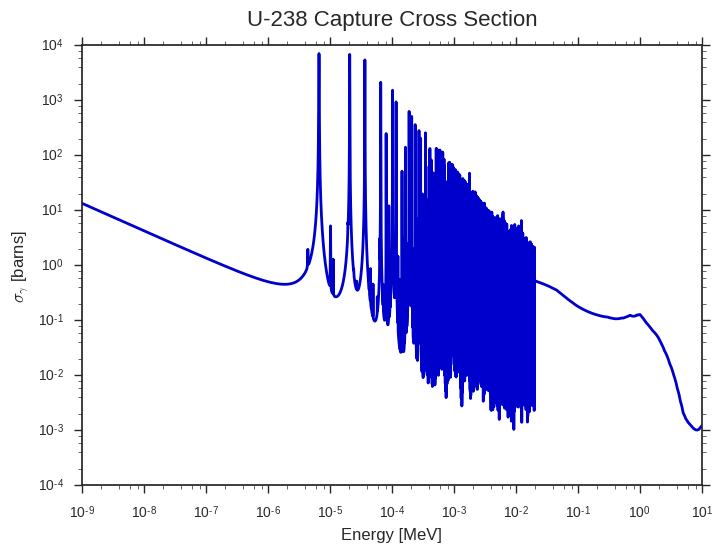
\includegraphics[width=0.8\linewidth]{figures/mgxs/u238-capture-xs}
\caption[U-238 capture cross section]{The continuous energy capture cross section for U-238.}
\label{fig:chap2-u238-xs}
\end{figure}
 
Although cross sections are experimentally measured, the neutron flux must be calculated analytically or with simulation. The steady-state Boltzmann transport equation~\cite{bell1970nuclear} is integro-differential in the neutron angular flux $\psi(\mathbf{r},\mathbf{\Omega},E)$ and balances the rate of change of the population of neutrons in phase space to the difference between the production and loss rates of neutrons within a closed system:

\begin{dmath}
\label{eqn:chap2-transport-ce}
\mathbf{\Omega} \cdot \nabla \psi(\mathbf{r},\mathbf{\Omega},E) + \Sigma_{t}(\mathbf{r},E)\psi(\mathbf{r},\mathbf{\Omega},E) \;\;\;\;\; = \;\;\;\;\; \int\displaylimits_{0}^{\infty}\int\displaylimits_{4\pi} \Sigma_{s}(\mathbf{r},{\mathbf{\Omega'}\rightarrow\mathbf{\Omega}},{E'\rightarrow E}) \psi(\mathbf{r},\mathbf{\Omega'},E') \mathrm{d}\mathbf{\Omega'} \mathrm{d}E' + Q(\mathbf{r},\mathbf{\Omega},E)
\end{dmath}

The first term on the left hand side of the equation represents the streaming of neutrons within space and the second term is the total neutron collision rate determined by the total cross section $\Sigma_{t}$. On the right hand side, the first term models the scattering of neutrons at energy $E'$ and direction $\mathbf{\Omega'}$ into some new energy $E$ and direction $\mathbf{\Omega}$. The final term represents a generic source $Q$ of neutrons. In the case of critical systems, such as nuclear reactors, $Q$ is a source of fission neutrons:

\begin{dmath}
\label{eqn:chap2-source}
Q(\mathbf{r},\mathbf{\Omega},E) = \frac{1}{k_{eff}}\int\displaylimits_{0}^{\infty}\int\displaylimits_{4\pi} \nu\Sigma_{f}(\mathbf{r},{\mathbf{\Omega'}\rightarrow \mathbf{\Omega}},{E'\rightarrow E})\psi(\mathbf{r},\mathbf{\Omega'},E') \mathrm{d}\mathbf{\Omega'} \mathrm{d}E'
\end{dmath}

The fission production cross section $\nu\Sigma_{f}$ represents the probability of neutrons of emitted at energy $E$ and angle $\mathbf{\Omega}$ resulting from fission events precipitated by neutrons at $E'$ and $\mathbf{\Omega'}$. The eigenvalue $k_{eff}$ of a critical system represents the multiplication of neutrons from fission and forces balance between neutron sources and losses due to absorption and leakage.

A solution for the neutron flux must computed from the transport equation. The accurate determination of the reaction rate distribution is primarily challenged by  the complicated energy structure of the cross sections. In addition, the distribution of neutrons in \ac{LWRs} spans 11 orders of magnitude from a few MeV at birth from fission emission to death by absorption at energies approaching 10$^{-5}$ eV. As a result, analytical solutions to Eqn.~\ref{eqn:chap2-transport-ce} are intractable without significant simplifying assumptions.

Instead, numerical simulation is used to solve the transport equation for the flux. Monte Carlo may be employed to exactly treat the energy dependence in Eqn.~\ref{eqn:chap2-transport-ce}\footnote{The treatment is only as exact as the uncertainties in measured nuclear cross section data will permit.}, but it is computationally burdensome and impractical for routine nuclear reactor analysis. Although space and angle may be discretized using standard techniques for the solution of PDEs, special treatment must be given to the energy variable. The following sections introduce approximations used to reduce the dimensionality of the equation to permit tractable multi-group calculations.

%The following sections present standard approximations made in multi-group theory to reduce the dimensionality of the angular, energy and spatial variables 


%%%%%%%%%%%%%%%%%%%%%%%%%%%%%%%%%%%%%%%%%%%%%%%%%%%%%%%%%%%%%%%%%%%%%%%%%%%%%%%
\section{Approximations in Angle}
\label{sec:chap2-approx-angle}

%%%%%%%%%%%%%%%%%%%%%%%%%%%
\subsection{Isotropic Fission Source}
\label{subsec:chap2-fiss-src}

The neutrons emitted from fission form a nearly isotropic distribution independent of the energy or angle of the incoming neutron. As a result, the fission production cross section can be approximated as $\nu\Sigma_{f}(\mathbf{r},{\mathbf{\Omega'}\rightarrow \mathbf{\Omega}},{E'\rightarrow E}) \approx \nu\Sigma_{f}(\mathbf{r},{E'\rightarrow E})$. This permits the fission source in Eqn.~\ref{eqn:chap2-source} to be written as:

\begin{dmath}
\label{eqn:chap2-source-scalar-flux}
Q(\mathbf{r},\mathbf{\Omega},E) = \frac{1}{4\pi k_{eff}}\int\displaylimits_{0}^{\infty}\int\displaylimits_{4\pi} \nu\Sigma_{f}(\mathbf{r},{E'\rightarrow E})\psi(\mathbf{r},\mathbf{\Omega'},E') \mathrm{d}\mathbf{\Omega'} \mathrm{d}E'
\end{dmath}

The isotropic approximation reduces the dimensionality of the fission production cross section and simplifies the derivation of the approximations in the following sections.

% such that $\nu\Sigma_{f}(\mathbf{r},{\Omega'\rightarrow \Omega},{E'\rightarrow E}) \approx \nu\Sigma_{f}(\mathbf{r},{E'\rightarrow E})$. 

% in terms of the scalar flux $\phi(\mathbf{r},E)$:

%\begin{dmath}
%\label{eqn:chap2-source-scalar-flux}
%Q(\mathbf{r},\mathbf{\Omega},E) = \frac{1}{4\pi k_{eff}} \int\displaylimits_{0}^{\infty}\nu\Sigma_{f}(\mathbf{r},{E'\rightarrow E})\phi(\mathbf{r},E') \mathrm{d}E'
%\end{dmath}

%\begin{dmath}
%\label{eqn:chap2-scalar-flux}
%\phi_{g}(\mathbf{r},E) = \int\displaylimits_{4\pi}\psi(\mathbf{r},\Omega,E)\mathrm{d}\Omega
%\end{dmath}


%%%%%%%%%%%%%%%%%%%%%%%%%%%%%%
\subsection{Angular Expansion of the Scattering Kernel}
\label{subsec:chap2-scatt-src}

Unlike the fission source, the scattering source cannot be treated as isotropic since it is strongly dependent on the relationship between the incoming and outgoing directions of motion. The dimensionality of the scattering source term in the transport equation -- known as the double differential scattering kernel -- is commonly reduced with basis function expansions in angle~\cite{hebert2009applied, cacuci2010handbook}. The angular flux is first expanded as an infinite sum of spherical harmonic functions $Y_{\ell}^{m}(\mathbf{\Omega})$ and angular flux moments $\psi_{\ell}^{m}$:

\begin{dmath}
\label{eqn:chap2-flux-expand}
\psi(\mathbf{r},\mathbf{\Omega},E) = \displaystyle\sum\limits_{\ell=0}^{\infty} \frac{2\ell+1}{4\pi} \displaystyle\sum\limits_{m=-\ell}^{\ell} \psi_{\ell}^{m}(\mathbf{r},E)Y_{l}^{m}(\mathbf{\Omega})
\end{dmath}

\begin{dmath}
\label{eqn:chap2-flux-moment}
\psi_{\ell}^{m}(\mathbf{r},E) = \displaystyle\int\limits_{4\pi} \psi(\mathbf{r},\mathbf{\Omega'},E)Y_{\ell}^{m}(\mathbf{\Omega'}) \mathrm{d}\Omega'
\end{dmath}

Similarly, the angular dependence of the scattering cross section $\Sigma_{s}(\mathbf{r},{\mathbf{\Omega'}\rightarrow\mathbf{\Omega}},{E'\rightarrow E})$ can be treated with a basis function expansion. The scattering cross section can be simplified without approximation by noting that the distribution over the change in direction $\mu$ is independent of the incoming angle $\mathbf{\Omega'}$ in scattering collisions. The re-parametrized scattering cross section $\Sigma_{s}(\mathbf{r},\mu,E'\rightarrow E)$ can then expanded as an infinite sum of Legendre polynomials $P_{\ell}(\mu)$ and scattering moments $\Sigma_{s,\ell}$:

\begin{dmath}
\label{eqn:chap2-scatt-expand}
\Sigma_{s}(\mathbf{r},\mu,E'\rightarrow E) = \displaystyle\sum\limits_{\ell=0}^{\infty} \frac{2\ell+1}{2} \displaystyle\sum\limits_{\ell=0}^{\infty}\Sigma_{s,\ell}(\mathbf{r},{E'\rightarrow E})P_{\ell}(\mu)
\end{dmath}

\begin{dmath}
\label{eqn:chap2-scatt-moment}
\Sigma_{s,\ell}(\mathbf{r},E'\rightarrow E) = \displaystyle\int\limits_{-1}^{1} \Sigma_{s}(\mathbf{r},\mu',{E\rightarrow E})P_{\ell}(\mu')\mathrm{d}\mu'
\end{dmath}

The expansions of the angular flux in spherical harmonics and scattering cross section in Legendre polynomials may be substituted into the scattering kernel. The spherical harmonic addition theorem can be applied to simplify the kernel in terms of only the real components $R_{l}^{m}$ of the spherical harmonics:

\begin{dmath}
\label{eqn:chap2-scatt-src-expand}
\int\displaylimits_{0}^{\infty}\int\displaylimits_{4\pi} \Sigma_{s}(\mathbf{r},{\mathbf{\Omega'}\rightarrow\mathbf{\Omega}},{E'\rightarrow E}) \psi(\mathbf{r},\mathbf{\Omega'},E') \mathrm{d}\mathbf{\Omega'} \mathrm{d}E' = \int\displaylimits_{0}^{\infty} \displaystyle\sum\limits_{\ell=0}^{\infty} \frac{2\ell+1}{4\pi} \displaystyle\sum\limits_{m=-\ell}^{\ell} \Sigma_{s,\ell}(\mathbf{r},{E'\rightarrow E}) \psi_{\ell}^{m}(\mathbf{r},E')R_{l}^{m}(\mathbf{\Omega}) \mathrm{d}E'
\end{dmath}

No approximation has been made to the scattering kernel's angular dependence in Eqn.~\ref{eqn:chap2-scatt-src-expand}. In practice, however, the expansion is truncated to a finite number of spherical harmonics $L$ to make the transport equation computationally tractable. The transport equation with the scattering source expansion and isotropic fission source is then:

\begin{dmath}
\label{eqn:chap2-transport-ce-2}
\mathbf{\Omega} \cdot \nabla \psi(\mathbf{r},\mathbf{\Omega},E) + \Sigma_{t}(\mathbf{r},E)\psi(\mathbf{r},\mathbf{\Omega},E) = \int\displaylimits_{0}^{\infty} \displaystyle\sum\limits_{\ell=0}^{\infty} \frac{2\ell+1}{4\pi} \displaystyle\sum\limits_{m=-\ell}^{\ell} \Sigma_{s,\ell}(\mathbf{r},{E'\rightarrow E}) \psi_{\ell}^{m}(\mathbf{r},E')R_{l}^{m}(\mathbf{\Omega}) \mathrm{d}E' + \frac{1}{4\pi k_{eff}}\int\displaylimits_{0}^{\infty}\int\displaylimits_{4\pi} \nu\Sigma_{f}(\mathbf{r},{E'\rightarrow E})\psi(\mathbf{r},\mathbf{\Omega'},E') \mathrm{d}\mathbf{\Omega'} \mathrm{d}E'
\end{dmath}


%%%%%%%%%%%%%%%%%%%%%%%%%%%%%%
\subsection{Transport Correction}
\label{subsec:chap2-transport-corr}

\cite{bell1970nuclear}\cite{macfarlane2000njoy}\cite{bell1967transport}

The scattering matrix and flux moments substantially increase the memory and storage requirements for calculation schemes which model anisotropic scattering with a finite moment expansion as introduced in Sec.~\ref{subsec:chap2-scatt-src}. One common approach to implicitly model anisotropic scattering is with transport corrected cross sections~\cite{bell1967transport,macfarlane1993transx,macfarlane2000njoy}. This approach first substitutes the angular flux expansion in Eqns.~\Crefrange{eqn:chap2-flux-expand}{eqn:chap2-flux-moment} into the total collision term in the transport equation:

\begin{dmath}
\label{eqn:chap2-tot-expand}
\Sigma_{t}(\mathbf{r},E)\psi(\mathbf{r},\mathbf{\Omega},E) = \displaystyle\sum\limits_{\ell=0}^{\infty} \frac{2\ell+1}{4\pi} \displaystyle\sum\limits_{m=-\ell}^{\ell} \Sigma_{t,\ell}^{m}(\mathbf{r},E) \psi_{\ell}^{m}(\mathbf{r},E)Y_{l}^{m}(\mathbf{\Omega})
\end{dmath}

\begin{dmath}
\label{eqn:chap2-tot-moment}
\Sigma_{t,\ell}^{m}(\mathbf{r},E) = \frac{\Sigma_{t}(\mathbf{r},E)\psi_{\ell}^{m}(\mathbf{r},E)}{\psi_{\ell}^{m}(\mathbf{r},E)}
\end{dmath}

The expanded total collision term in Eqn.~\ref{eqn:chap2-tot-expand} can be moved to the right hand side of Eqn.~\ref{eqn:chap2-transport-ce-2}, and with some simplifications, incorporated into the scattering kernel expansion. A new free parameter for the transport corrected total cross section $\Sigma_{tr}$ is then added as a reaction rate to each side of the transport equation, where the spatial and energy variables have been dropped for simplicity:

\begin{dmath}
\label{eqn:chap2-transport-ce-3}
\mathbf{\Omega} \cdot \nabla \psi + \Sigma_{tr}\psi = \int\displaylimits_{0}^{\infty} \displaystyle\sum\limits_{\ell=0}^{L} \frac{2\ell+1}{4\pi} \displaystyle\sum\limits_{m=-\ell}^{\ell} \left(\Sigma_{s,\ell} - \left(\Sigma_{t,\ell}^{m} - \Sigma_{tr}\right)\delta_{E',E}\right) \psi_{\ell}^{m}R_{l}^{m}(\mathbf{\Omega}) \mathrm{d}E' + \frac{1}{4\pi k_{eff}}\int\displaylimits_{0}^{\infty}\int\displaylimits_{4\pi} \nu\Sigma_{f}\psi \mathrm{d}\mathbf{\Omega'} \mathrm{d}E'
\end{dmath}

The scattering kernel expansion has been truncated to order $L$ and the variable $\delta_{E',E}$ is the Kronecker delta function. A variety of forms for the transport cross section $\Sigma_{tr}$ are extensively discussed in the literature. One of the most commonly used versions of $\Sigma_{tr}$ is known as the \textit{in-scatter approximation}~\cite{yamamoto2008simplified}. In the case of isotropic scattering where $L = 0$, the in-scatter approximation is defined as the total cross section with a current-weighted correction term based on $\Sigma_{s,\ell=1}$:

%This form is Each of these forms are presented here for the case of isotropic scattering where $L = 0$, as is a common scenario in many deterministic transport codes.

\begin{dmath}
\label{eqn:chap2-transport-in-scatt-curr}
\Sigma_{tr}(\mathbf{r},E) \equiv \Sigma_{t}(\mathbf{r},E) - \frac{\int\limits_{0}^{\infty}\Sigma_{s,\ell=1}(\mathbf{r},{E'\rightarrow E})\psi_{1}(\mathbf{r},E')\mathrm{d}E'}{\psi_{1}(\mathbf{r},E)}
\end{dmath}

Since it is generally impractical to compute the neutron current \textit{a priori}, the first moment of the flux -- known as the scalar flux $\phi$ -- is more commonly used to weight the correction term:

%In-scatter approximation with scalar flux weighting - make the approximation that weighting with the current $\psi_{1}$ is akin to weighting with the scalar flux $\psi_{0}$:

\begin{dmath}
\label{eqn:chap2-transport-in-scatt-flux}
\Sigma_{tr}(\mathbf{r},E) \equiv \Sigma_{t}(\mathbf{r},E) - \frac{\int\limits_{0}^{\infty}\Sigma_{s,\ell=1}(\mathbf{r},{E'\rightarrow E})\psi_{0}(\mathbf{r},E')\mathrm{d}E'}{\psi_{0}(\mathbf{r},E)}
\end{dmath}

%Out-scatter approximation:

%\begin{dmath}
%\label{eqn:chap2-transport-out-scatt}
%\Sigma_{tr}(\mathbf{r},E) \equiv \Sigma_{t}(\mathbf{r},E) - \int\limits_{0}^{\infty}%\Sigma_{s,\ell=1}(\mathbf{r},{E'\rightarrow E})\mathrm{d}E'
%\end{dmath}

%\begin{itemize}[noitemsep]
%  \item present consistent-p approx.
%  \item present our form of the transport correction
%  \item talk about isotropic scattering approx. in deterministic codes
%\end{itemize}


Although some deterministic transport codes explicitly treat the anisotropy of the scattering source with a finite moment expansion, it is common for many methods to assume isotropic scattering and model the first term in the expansion in terms of the scalar neutron flux $\phi$:

\begin{dmath}
\label{eqn:chap2-scatt-src-iso}
\int\displaylimits_{0}^{\infty}\int\displaylimits_{4\pi} \Sigma_{s}(\mathbf{r},{\mathbf{\Omega'}\rightarrow\mathbf{\Omega}},{E'\rightarrow E}) \psi(\mathbf{r},\mathbf{\Omega'},E') \mathrm{d}\mathbf{\Omega'} \mathrm{d}E' \approx \frac{1}{4\pi} \int\displaylimits_{0}^{\infty} \Sigma_{s}(\mathbf{r},{E'\rightarrow E}) \psi_{0}(\mathbf{r},E') = \frac{1}{4\pi} \int\displaylimits_{0}^{\infty} \Sigma_{s,0}(\mathbf{r},{E'\rightarrow E}) \phi(\mathbf{r},E') \mathrm{d}E'
\end{dmath}

\begin{dmath}
\label{eqn:chap2-source-scalar-flux}
\phi(\mathbf{r},E) = \int\displaylimits_{4\pi}\psi(\mathbf{r},\mathbf{\Omega'},E) \mathrm{d}\Omega'
\end{dmath}



%%%%%%%%%%%%%%%%%%%%%%%%%%%%%%%%%%%%%%%%%%%%%%%%%%%%%%%%%%%%%%%%%%%%%%%%%%%%%%%
\section{Approximations in Energy}
\label{sec:chap2-approx-energy}

%%%%%%%%%%%%%%%%%%%%%%%%%%%%%%%%%%
\subsection{Energy Discretization}
\label{subsec:chap2-energy}

The multi-group approach used to solve the transport equation subdivides the neutron's energy into discrete bins known as energy groups. The energy groups are indexed starting at 1 for high energies and ending with $G$ for the lowest energies of interest. An energy group $g \in \left\{1, 2, \ldots, G\right\}$  spans a range of energies from $\left[E_{g}, E_{g-1}\right]$ where $E_{0}$ is the lowest energy under consideration\footnote{Although $E_{0}$ is often taken to be zero, this may not be appropriate in practice since cross sections can only be accurately measured for finite neutron energies.} and $E_{g}$ is the upper bound of group $g$. First, a group-wise angular flux $\psi_{g}$ is defined for each energy group:

\begin{dmath}
\label{eqn:chap2-groupwise-flux}
\psi_{g}(\mathbf{r},\mathbf{\Omega}) = \int\displaylimits_{E_{g}}^{E_{g-1}} \psi(\mathbf{r},\mathbf{\Omega},E)\mathrm{d}E
\end{dmath}

%A group-wise scalar flux $\phi_{g}$ can be similarly defined.

Next, the continuous energy transport equation (Eqn.~\ref{eqn:chap2-transport-ce}) with a fission source (Eqn.~\ref{eqn:chap2-source}) can be transformed into its multi-group form by first integrating over each energy group:

\begin{dmath}
\label{eqn:chap2-transport-mg-1}
\mathbf{\Omega} \cdot \nabla \psi_{g}(\mathbf{r},\mathbf{\Omega}) + \int\displaylimits_{E_{g}}^{E_{g-1}} \Bigg[\Sigma_{t}(\mathbf{r},E)\psi(\mathbf{r},\mathbf{\Omega},E)\Bigg]\mathrm{d}E = \;\;\; \int\displaylimits_{E_{g}}^{E_{g-1}} \Bigg[\sum_{g'=1}^{G} \int\displaylimits_{E_{g'}}^{E_{g'-1}}\int\displaylimits_{4\pi} \Sigma_{s}(\mathbf{r},{\mathbf{\Omega'}\rightarrow\mathbf{\Omega}},{E'\rightarrow E}) \psi(\mathbf{r},\mathbf{\Omega'},E') \mathrm{d}\mathbf{\Omega'} \mathrm{d}E'\Bigg]\mathrm{d}E + 
\int\displaylimits_{E_{g}}^{E_{g-1}}\Bigg[\frac{1}{4\pi k_{eff}}\sum_{g'=1}^{G} \int\displaylimits_{E_{g'}}^{E_{g'-1}}\int\displaylimits_{4\pi}\nu\Sigma_{f}(\mathbf{r},{E'\rightarrow E})\psi(\mathbf{r},\mathbf{\Omega'},E')\mathrm{d}\mathbf{\Omega'}\mathrm{d}E'\Bigg]\mathrm{d}E
\end{dmath}

The integrals in Eqn.~\ref{eqn:chap2-transport-mg-1} over incoming neutron energy in the scattering kernel and fission source are treated as summations of discrete integrals over each incoming energy group. 


Although the streaming term is easily expressed in terms of the multi-group flux $\psi_{g}$, the total collision, scattering and fission terms are defined as integral quantities. These three terms can be simplified by multiplying each by unity in the form of $\nicefrac{\psi_{g}}{\psi_{g}}$:

\begin{dmath}
\label{eqn:chap2-transport-mg-2}
\mathbf{\Omega} \cdot \nabla \psi_{g}(\mathbf{r},\mathbf{\Omega}) + \ddfrac{\int\displaylimits_{E_{g}}^{E_{g-1}} \Sigma_{t}(\mathbf{r},E)\psi(\mathbf{r},\mathbf{\Omega},E)\mathrm{d}E}{\psi_{g}(\mathbf{r},\mathbf{\Omega})}\psi_{g}(\mathbf{r},\mathbf{\Omega}) 
= \;\;\; 
\sum_{g'=1}^{G} \ddfrac{\int\displaylimits_{E_{g}}^{E_{g-1}} \int\displaylimits_{E_{g'}}^{E_{g'-1}}\int\displaylimits_{4\pi} \Sigma_{s}(\mathbf{r},{\mathbf{\Omega'}\rightarrow\mathbf{\Omega}},{E'\rightarrow E}) \psi(\mathbf{r},\mathbf{\Omega'},E') \mathrm{d}\mathbf{\Omega'} \mathrm{d}E'}{\psi_{g'}(\mathbf{r},\mathbf{\Omega'})}\psi_{g'}(\mathbf{r},\mathbf{\Omega'})
+ 
\dfrac{1}{4\pi k_{eff}} \sum_{g'=1}^{G} \ddfrac{\int\displaylimits_{E_{g}}^{E_{g-1}} \int\displaylimits_{E_{g'}}^{E_{g'-1}}\int\displaylimits_{4\pi} \nu\Sigma_{f}(\mathbf{r},{E'\rightarrow E})\psi(\mathbf{r},\mathbf{\Omega'},E') \mathrm{d}\mathbf{\Omega'} \mathrm{d}E'\mathrm{d}E}{\psi_{g'}(\mathbf{r},\mathbf{\Omega'})}\psi_{g'}(\mathbf{r},\mathbf{\Omega'})
\end{dmath}

The fractional terms in the Eqn.~\ref{eqn:chap2-transport-mg-2} are defined as the \ac{MGXS} for total, scattering and fission production reactions. The \ac{MGXS} are the averages of the corresponding continuous energy cross sections weighted by the angular neutron flux $\psi$ in each energy group. The \ac{MGXS} $\Sigma_{t,g}$, $\Sigma_{s,g' \rightarrow g}$ and $\nu\Sigma_{f,g' \rightarrow g}$ are defined below for completeness:

\begin{dmath}
\label{eqn:chap2-sigt-mg}
\Sigma_{t,g}(\mathbf{r},\mathbf{\Omega}) \equiv \frac{\int\displaylimits_{E_{g}}^{E_{g-1}} \Sigma_{t}(\mathbf{r},E)\psi(\mathbf{r},\mathbf{\Omega},E)\mathrm{d}E}{\psi_{g}(\mathbf{r},\mathbf{\Omega})}
\end{dmath}

\begin{dmath}
\label{eqn:chap2-sigs-mg}
\Sigma_{s,g' \rightarrow g}(\mathbf{r},\mathbf{\Omega}) \equiv \frac{\int\displaylimits_{E_{g}}^{E_{g-1}} \int\displaylimits_{E_{g'}}^{E_{g'-1}}\int\displaylimits_{4\pi} \Sigma_{s}(\mathbf{r},{\mathbf{\Omega'}\rightarrow\mathbf{\Omega}},{E'\rightarrow E}) \psi(\mathbf{r},\mathbf{\Omega'},E') \mathrm{d}\mathbf{\Omega'} \mathrm{d}E' \mathrm{d}E} {\psi_{g'}(\mathbf{r},\mathbf{\Omega'})}
\end{dmath}

\begin{dmath}
\label{eqn:chap2-nusigf-mg}
\nu\Sigma_{f,g' \rightarrow g}(\mathbf{r},\mathbf{\Omega}) \equiv \frac{\int\displaylimits_{E_{g}}^{E_{g-1}} \int\displaylimits_{E_{g'}}^{E_{g'-1}}\int\displaylimits_{4\pi} \nu\Sigma_{f}(\mathbf{r},{E'\rightarrow E})\psi(\mathbf{r},\mathbf{\Omega'},E') \mathrm{d}\mathbf{\Omega'} \mathrm{d}E'\mathrm{d}E}{\psi_{g'}(\mathbf{r},\mathbf{\Omega'})}
\end{dmath}

With these definitions of the \ac{MGXS}, the multi-group form of the transport equation in Eqn.~\ref{eqn:chap2-transport-mg-1} can be expressed succinctly in terms of the group-wise angular flux $\psi_{g}$:

\begin{dmath}
\label{eqn:chap2-transport-mg-3}
\mathbf{\Omega} \cdot \nabla \psi_{g}(\mathbf{r},\mathbf{\Omega}) + \Sigma_{t,g}(\mathbf{r},E)\psi_{g}(\mathbf{r},\mathbf{\Omega}) =
\sum_{g'=1}^{G} \int\displaylimits_{4\pi} \Sigma_{s,g' \rightarrow g}(\mathbf{r},{\mathbf{\Omega'}\rightarrow\mathbf{\Omega}}) \psi_{g}(\mathbf{r},\mathbf{\Omega'}) \mathrm{d}\mathbf{\Omega'} + \frac{1}{4\pi k_{eff}}\sum_{g'=1}^{G} \int\displaylimits_{4\pi} \nu\Sigma_{f,g' \rightarrow g}(\mathbf{r})\psi_{g}(\mathbf{r},\mathbf{\Omega'}) \mathrm{d}\mathbf{\Omega'}
\end{dmath}

Thus far, no approximations have been made in the energy discretization of multi-group transport equation given in Eqn.~\ref{eqn:chap2-transport-mg-3}. However, the expressions for the \ac{MGXS} $\Sigma_{t,g}$, $\Sigma_{s,g' \rightarrow g}$ and $\nu\Sigma_{f,g' \rightarrow g}$ in Eqns.~\Crefrange{eqn:chap2-sigt-mg}{eqn:chap2-nusigf-mg} present a complication since they are dependent on the unknown angular flux as discussed in the following section.

-should I expand in angular moments first?\\
-it's not appropriate to simply remove the energy dependence in the scattering cross section is it?\\


%%%%%%%%%%%%%%%%%%%%%%%%%%%%%%
\subsection{Flux Separability Approximation}
\label{subsec:chap2-angle}

The angular dependence of the \ac{MGXS} is commonly treated with the flux separability approximation. Flux separability makes the simplifying assumption that the energy and angular dependence of the flux varies independently such that the angular flux can be written as the product of the scalar neutron flux $\phi(\mathbf{r},E)$ and some function $W(\mathbf{r}, \mathbf{\Omega})$:

\begin{dmath}
  \label{eqn:chap2-flux-separate}
  \psi(\mathbf{r},\mathbf{\Omega},E) = \phi(\mathbf{r},E) W(\mathbf{r},\mathbf{\Omega})
\end{dmath}

\begin{dmath}
\label{eqn:chap2-scalar-flux}
\phi(\mathbf{r},E) = \int\displaylimits_{4\pi} \psi(\mathbf{r},\mathbf{\Omega},E)\mathrm{d}\mathbf{\Omega}
\end{dmath}

The angular dependence of the \ac{MGXS} is eliminated by inserting Eqn.~\ref{eqn:chap2-flux-separate} into Eqns.~\cref{eqn:chap2-sigt-mg,eqn:chap2-sigs-mg,eqn:chap2-nusigf-mg}, factoring out $W(\mathbf{r}, \mathbf{\Omega})$ and writing the \ac{MGXS} in terms of the scalar flux:

% $\phi(\mathbf{r},E)$:

\begin{dmath}
\label{eqn:chap2-sigt-mg-scalar}
\Sigma_{t,g}(\mathbf{r}) \equiv \frac{\int\displaylimits_{E_{g}}^{E_{g-1}} \Sigma_{t}(\mathbf{r},E)\phi(\mathbf{r},E)\mathrm{d}E}{\phi_{g}(\mathbf{r})}
\end{dmath}

\begin{dmath}
\label{eqn:chap2-sigs-mg-scalar}
\Sigma_{s,g' \rightarrow g}(\mathbf{r}) \equiv \frac{\int\displaylimits_{E_{g}}^{E_{g-1}} \int\displaylimits_{E_{g'}}^{E_{g'-1}} \Sigma_{s}(\mathbf{r},{E'\rightarrow E}) \phi(\mathbf{r},E') \mathrm{d}E' \mathrm{d}E} {\phi_{g'}(\mathbf{r})}
\end{dmath}

\begin{dmath}
\label{eqn:chap2-nusigf-mg-scalar}
\nu\Sigma_{f,g' \rightarrow g}(\mathbf{r}) \equiv \frac{\int\displaylimits_{E_{g}}^{E_{g-1}} \int\displaylimits_{E_{g'}}^{E_{g'-1}} \nu\Sigma_{f}(\mathbf{r},{E'\rightarrow E})\phi(\mathbf{r},E') \mathrm{d}E'\mathrm{d}E}{\phi_{g'}(\mathbf{r})}
\end{dmath}

%The group-wise scalar flux $\phi_{g}$ is the corollary to its angle dependent counterpart $\psi_{g}$:

%\begin{dmath}
%\label{eqn:chap2-scalar-flux-mg}
%\phi_{g}(\mathbf{r}) = \int\displaylimits_{E_{g}}^{E_{g-1}}\phi(\mathbf{r},E)\mathrm{d}E
%\end{dmath}

-mention that this approx. will be reivisited in later sections\\
-refer to consistent-p approximation \\
-cite nuclear eng handbook?\\


%%%%%%%%%%%%%%%%%%%%%%%%%%%%%%%%%%%
\subsection{Scattering Production}
\label{sec:chap2-scatt-prod}

Although neutron production is dominated by fission in nuclear reactors, there may also be non-negligible production of neutrons due to scattering multiplicity $(n,xn)$ reactions. Production from scattering is typically accounted for with a factor $\nu_{scatt,i,g' \rightarrow g}$ which represents the average number of neutrons produced in a scattering reaction. The factor $\nu_{scatt,i,g' \rightarrow g}$ may be lumped into the scattering matrix $\nu_{scatt,i,g' \rightarrow g}\Sigma_{s,i,g' \rightarrow g}$ and substituted directly into the scattering source term in the multi-group transport equation. 

The $k_{eff}$ eigenvalue is only defined for fission operator in the transport equation. As a result, deterministic methods which compute the eigenvalue using the fission production, absorption and leakage rates will fail to capture the scattering production in in the multiplication factor. In order to account for $(n,xn)$ reactions, a ``corrected'' absorption cross section $\tilde{\Sigma}_{a,i,g} = \Sigma_{a,i,g} - (1-\nu_{scatt,i,g' \rightarrow g})\Sigma_{s,i,g' \rightarrow g}$ must be used to preserve neutron balance. Alternatively, $(n,xn)$ reactions will be accounted for if the eigenvalue is computed as the ratio of successive fission sources in iterative deterministic methods.


%%%%%%%%%%%%%%%%%%%%%%%%%%%%%%%%%%%
\subsection{Fission Matrix Condensation}
\label{sec:chap2-fiss-mat}

The scattering and fission production matrices dominate the memory storage requirements for \ac{MGXS} since they depend on both incoming and outgoing energy groups. In thermal reactors the energy distribution of neutrons produced in fission is nearly independent of the incoming neutron energy, and the fission production matrix can be condensed into two single dimensional vectors for each energy group. The fission spectrum $\chi_{g}$ is introduced as a probability distribution over outgoing fission energies:

\begin{dmath}
\label{eqn:chap2-nusifg}
\chi_{g} \equiv \frac{\displaystyle\sum\limits_{g'=1}^{G}\nu\Sigma_{f,g'\rightarrow g}\phi_{g'}}{\displaystyle\sum\limits_{g=1}^{G}\displaystyle\sum\limits_{g'=1}^{G}\nu\Sigma_{f,g'\rightarrow g}}
\end{dmath}

The group-wise fission production cross section $\nu\Sigma_{f,g}$ is defined as the flux-weighted sum of $\nu\Sigma_{f,g'\rightarrow g}$ over all outgoing groups:

% and signifies the probability of fission occurring in group $g$:

\begin{dmath}
\label{eqn:chap2-nusifg}
\nu\Sigma_{f,g'} \equiv \displaystyle\sum\limits_{g'=1}^{G}\nu\Sigma_{f,g'\rightarrow g}\phi_{g'}
\end{dmath}

Upon substituting $\chi_{g}$ and $\nu\Sigma_{f,g}$ into Eqn.~\ref{eqn:chap2-transport-mg-4} one obtains:

\begin{dmath}
\label{eqn:chap2-transport-mg-6}
\mathbf{\Omega} \cdot \nabla \psi_{g}(\mathbf{r},\mathbf{\Omega}) + \Sigma_{t,i,g}\psi_{g}(\mathbf{r},\mathbf{\Omega}) \;\;\;\; = \;\;\;\;\;
\sum_{g'=1}^{G} \int\displaylimits_{4\pi} \Sigma_{s,i,g' \rightarrow g}(\mathbf{r},{\mathbf{\Omega'}\rightarrow\mathbf{\Omega}}) \psi_{g}(\mathbf{r},\mathbf{\Omega'}) \mathrm{d}\mathbf{\Omega'} + 
\frac{\chi_{i,g}}{4\pi k_{eff}}\sum_{g'=1}^{G} \int\displaylimits_{4\pi} \nu\Sigma_{f,i,g}\psi_{g}(\mathbf{r},\mathbf{\Omega'}) \mathrm{d}\mathbf{\Omega'}
\end{dmath}


%frequently made in multi-group transport calculations thermal reactor spectra the energy distribution of neutrons produced in fission is nearly independent of the incoming neutron energy.

%to reduce the dimensionality of the fission production matrix $\nu\Sigma_{f,g'\rightarrow g}$. In thermal reactor spectra the energy distribution of neutrons produced in fission is nearly independent of the incoming neutron energy.


%%%%%%%%%%%%%%%%%%%%%%%%%%%%%%%%%%%%%%%%%%%%%%%%%%%%%%%%%%%%%%%%%%%%%%%%%%%%%%%
\section{Approximations in Space}
\label{sec:chap2-approx-space}

%%%%%%%%%%%%%%%%%%%%%%%%%%%%%%%%%%%
\subsection{Spatial Homogenization}
\label{subsec:chap2-space}

%Up to this point the \ac{MGXS} have been defined as continuously varying in space. Most deterministic methods solve the multi-group transport equation by discretizing the spatial domain. The following equation introduces an integral over each mesh cell $i$ to each term in the multi-group transport equation:

%\begin{dmath}
%\label{eqn:chap2-transport-mg-4}
%\int\displaylimits_{\mathbf{r} \in V_{i}}\left(\mathbf{\Omega} \cdot \nabla \psi_{g}(\mathbf{r},\mathbf{\Omega}) + \Sigma_{t,g}(\mathbf{r})\psi_{g}(\mathbf{r},\mathbf{\Omega})\right)\mathrm{d}\mathbf{r} \;\;\;\; = \;\;\;\;\; \int\displaylimits_{\mathbf{r} \in V_{i}}\sum_{g'=1}^{G} \int\displaylimits_{4\pi} \Sigma_{s,g' \rightarrow g}(\mathbf{r},{\mathbf{\Omega'}\rightarrow\mathbf{\Omega}}) \psi_{g}(\mathbf{r},\mathbf{\Omega'}) \mathrm{d}\mathbf{\Omega'} \mathrm{d}\mathbf{r} + \frac{1}{4\pi k_{eff}}\int\displaylimits_{\mathbf{r} \in V_{i}}\sum_{g'=1}^{G} \int\displaylimits_{4\pi} \nu\Sigma_{f,g' \rightarrow g}(\mathbf{r})\psi_{g}(\mathbf{r},\mathbf{\Omega'}) \mathrm{d}\mathbf{\Omega'} \mathrm{d}\mathbf{r}
%\end{dmath}

Up to this point the \ac{MGXS} have been defined as continuously varying in space. In practice, most deterministic methods used to solve the multi-group transport equation make the simplifying assumption that the material properties are constant across each mesh cell. Spatial homogenization is used to to compute flux-weighted volume-averaged cross sections within each mesh cell $i$ with volume $V_{i}$ as follows:

\begin{dmath}
\label{eqn:chap2-sigt-mg-scalar}
\Sigma_{t,i,g} = \frac{\int\displaylimits_{\mathbf{r} \in V_{i}}\int\displaylimits_{E_{g}}^{E_{g-1}} \Sigma_{t}(\mathbf{r},E)\phi(\mathbf{r},E)\mathrm{d}E\mathrm{d}\mathbf{r}}{\int\displaylimits_{\mathbf{r} \in V_{i}}\phi_{g}(\mathbf{r})\mathrm{d}\mathbf{r}}
\end{dmath}

\begin{dmath}
\label{eqn:chap2-sigs-mg-scalar}
\Sigma_{s,i,g' \rightarrow g} \equiv \frac{\int\displaylimits_{\mathbf{r} \in V_{i}}\int\displaylimits_{E_{g}}^{E_{g-1}} \int\displaylimits_{E_{g'}}^{E_{g'-1}} \Sigma_{s}(\mathbf{r},{E'\rightarrow E}) \phi(\mathbf{r},E') \mathrm{d}E' \mathrm{d}E\mathrm{d}\mathbf{r}}{\int\displaylimits_{\mathbf{r} \in V_{i}}\phi_{g'}(\mathbf{r})\mathrm{d}\mathbf{r}}
\end{dmath}

\begin{dmath}
\label{eqn:chap2-nusigf-mg-scalar}
\nu\Sigma_{f,i,g' \rightarrow g} \equiv \frac{\int\displaylimits_{\mathbf{r} \in V_{i}}\int\displaylimits_{E_{g}}^{E_{g-1}} \int\displaylimits_{E_{g'}}^{E_{g'-1}} \nu\Sigma_{f}(\mathbf{r},{E'\rightarrow E})\phi(\mathbf{r},E') \mathrm{d}E'\mathrm{d}E\mathrm{d}\mathbf{r}}{\int\displaylimits_{\mathbf{r} \in V_{i}}\phi_{g'}(\mathbf{r})\mathrm{d}\mathbf{r}}
\end{dmath}

A variety of discretization schemes may be used to solve the following multi-group transport equation in Eqn.~\ref{eqn:chap2-transport-mg-3}, including the \ac{MOC} and discrete ordinates (S$_N$). For first order discretization schemes in space, the transport equation can be re-written in terms of the volume-averaged group-wise fluxes $\psi_{i,g}$ and the spatially homogenized \ac{MGXS} in each mesh cell and energy group:

\begin{dmath}
\label{eqn:chap2-transport-mg-4}
\mathbf{\Omega} \cdot \nabla \psi_{i,g}(\mathbf{\Omega}) + \Sigma_{t,i,g}\psi_{i,g}(\mathbf{\Omega}) \;\;\;\; = \;\;\;\;\;
\sum_{g'=1}^{G} \int\displaylimits_{4\pi} \Sigma_{s,i,g' \rightarrow g}({\mathbf{\Omega'}\rightarrow\mathbf{\Omega}}) \psi_{i,g}(\mathbf{\Omega'}) \mathrm{d}\mathbf{\Omega'} + 
\frac{1}{4\pi k_{eff}}\sum_{g'=1}^{G} \int\displaylimits_{4\pi} \nu\Sigma_{f,i,g' \rightarrow g}\psi_{i,g}(\mathbf{\Omega'}) \mathrm{d}\mathbf{\Omega'}
\end{dmath}

This is the form of the multi-group transport equation solved using the deterministic OpenMOC code in this thesis. 


\begin{itemize}[noitemsep]
  \item equation and figures mapped to variables
  \item tally ``noise'' model
  \item uncertainty propagation equations
  \item mention that this intro is agnostic to the method used to solve the transport eqn.
   \item mention recent work to use MC for MGXS (chap. 3 of nelson's thesis)
   \item figure 2.2 from adam's thesis to describe typical approach
\end{itemize}


%%%%%%%%%%%%%%%%%%%%%%%%%%%
\subsection{Approximations}
\label{subsec:chap2-approx}

%%%%%%%%%%%%%%%%%%%%%%%%%%%%%%%%%%%%
\subsubsection{Isotropic Scattering}
\label{subsubsec:chap2-iso-scatter}

\begin{itemize}
  \item mention ``iso-in-lab'' feature in OpenMC
\end{itemize}


%%%%%%%%%%%%%%%%%%%%%%%%%%%%%%%%%%%%%%%%%%%%%%%%%%%%%%%%%%%%%%%%%%%%%%%%%%%%%%%
\section{MGXS Generation with Monte Carlo}
\label{sec:chap2-mgxs-mc}

\begin{itemize}[noitemsep]
  \item \ac{MC} is \emph{reactor agnostic}
  \item stochastic approx. to integrals in Section~\ref{sec:chap2-background}
\end{itemize}

%%%%%%%%%%%%%%%%%%%%%%
\subsection{Past Work}
\label{subsec:chap2-past-work}

\begin{itemize}[noitemsep]
  \item \ac{MGXS} for coarse mesh diffusion
  \begin{itemize}[noitemsep]
    \item Redmond
    \item Pounders
    \item Serpent
  \end{itemize}
  \item \ac{MGXS} for fine mesh transport
  \begin{itemize}[noitemsep]
    \item Nelson with NDPP
  \end{itemize}
\end{itemize}

%%%%%%%%%%%%%%%%%%%%%%%%%%%%%%%%%%%%%%%%%%%%%
\subsection{Spatial Self-Shielding Treatment}
\label{subsec:chap2-spatial-shield}

\begin{itemize}[noitemsep]
  \item spatial self-shielding treatment is natural in \ac{MC}
  \item challenge is slow convergence rate
  \item motivate clustering
\end{itemize}